%! Mode:: "TeX:UTF-8"
%! TEX program = xelatex
\PassOptionsToPackage{quiet}{xeCJK}
\documentclass[withoutpreface,bwprint]{cumcmthesis}
\usepackage{etoolbox}
\BeforeBeginEnvironment{tabular}{\zihao{-5}}
\usepackage[numbers,sort&compress]{natbib}  % 文献管理宏包
\usepackage[framemethod=TikZ]{mdframed}  % 框架宏包
\usepackage{url}  % 网页链接宏包
\usepackage{subcaption}  % 子图宏包
\usepackage{tabularx}  % 宽表格自适应
\usepackage{booktabs}  % \\toprule/\\midrule/\\bottomrule
\usepackage[table]{xcolor}  % 表格行配色与 \\rowcolors
\allowdisplaybreaks[4]
\newcolumntype{C}{>{\centering\arraybackslash}X}
\newcolumntype{R}{>{\raggedleft\arraybackslash}X}
\newcolumntype{L}{>{\raggedright\arraybackslash}X}

\title{基于模型预测控制(MPC)与遗传算法(GA)的网络切片分配优化}  % 论文标题
\tihao{}  % 题号
\baominghao{}  % 报名号
\schoolname{}  % 学校
\membera{}  % 队员a
\memberb{}  % 队员b
\memberc{}  % 队员c
\supervisor{}  % 指导老师
\yearinput{}
\monthinput{}
\dayinput{}

%%%%%%%%%%%%%%%%%%%%%%%%%%%%%%%%%%%%%%%%%%%%%%%%%%%%%%%%%%%%%
%% 正文
\begin{document}

\maketitle
\begin{abstract}
随着物联网设备的指数级增长,移动通信需求呈现爆发式增长,推动了网络架构的不断演进。本文针对无线网络切片资源管理的一系列复杂优化问题,设计并实现了一套从静态到动态、从同构到异构、从性能优先到兼顾能耗的渐进式求解方案。

\textbf{对于问题一,} 我们针对单基站静态场景,建立了服务质量(QoS)最大化模型。通过对所有可能的资源块(RB)分配方案进行穷举搜索,得到了全局最优解:为URLLC、eMBB、mMTC切片分别分配\textbf{20、10、20}个RB时,可达到最大QoS得分\textbf{15.78}。此结果为后续更复杂的问题提供了性能基准。

\textbf{对于问题二,} 面对动态任务到达和时变信道,我们引入了\textbf{模型预测控制(MPC)}框架。将总时长划分为10个100ms的决策窗口,在每个窗口开始时,根据当前系统状态(如用户队列)进行枚举寻优。该方法有效应对了系统的动态性,实现了\textbf{337.42}的累计QoS,验证了MPC框架处理时变问题的有效性。

\textbf{对于问题三,} 在存在同频干扰的多微基站场景下,决策维度急剧增加。我们建立了用户接入、RB分配和功率控制的联合优化模型,并提出一种\textbf{MPC结合遗传算法(GA)}的两层求解框架。外层MPC负责时域滚动,内层GA通过混合编码方案,高效求解每个窗口内非凸、高维的静态资源分配问题,最终在有效抑制干扰的同时,获得了\textbf{853.37}的累计QoS。

\textbf{对于问题四,} 针对宏基站(MBS)与微基站(SBS)共存的异构网络,我们对MPC+GA框架进行了扩展。模型引入异构网络下的MBS与SBS资源分配和功率控制,以及用户只能接入MBS或最近SBS的约束。求解结果显示出智能的\textbf{网络功能协同策略}:无干扰、资源丰富的MBS主要承载海量mMTC连接,而靠近用户的SBS则重点保障URLLC等高性能业务,最终将累计QoS提升至\textbf{1041.28}。

\textbf{对于问题五,} 为在保障QoS的同时最小化网络能耗,我们设计了一种新颖的\textbf{两阶段优化算法}。在MPC框架的每个窗口内,第一阶段采用GA优化发射功率以最小化能耗;第二阶段在给定功率下,通过枚举优化RB分配以最大化QoS。该分层解耦策略成功平衡了性能与能耗的矛盾,在将总能耗控制在\textbf{183.68}焦耳的同时,取得了\textbf{381.17}的累计QoS。

综上,本文通过对一系列问题的层层递进的建模与求解,系统地展示了如何运用枚举、MPC、遗传算法及分层优化等方法,解决不同复杂度下的网络切片资源管理难题,为设计高效、智能的无线资源分配方案提供了有价值的思路与验证。

\keywords{ 模型预测控制(MPC)\quad 遗传算法(GA)\quad 异构网络\quad 两阶段优化算法}
\end{abstract}
%%%%%%%%%%%%%%%%%%%%%%%%%%%%%%%%%%%%%%%%%%%%%%%%%%%%%%%%%%%%% 

\tableofcontents  % 目录
\newpage

%%%%%%%%%%%%%%%%%%%%%%%%%%%%%%%%%%%%%%%%%%%%%%%%%%%%%%%%%%%%%  
\section{问题重述}
\subsection{问题背景}
随着移动通信需求的激增和物联网(IoT)的快速发展,网络架构正向异构化和虚拟化演进。异构蜂窝网络(HetNet)通过混合部署宏基站与微基站,有效提升了网络容量与覆盖。在此基础上,5G网络切片技术利用网络功能虚拟化(NFV),将单一物理网络划分为多个逻辑切片,以满足超高可靠低时延(URLLC)、增强移动宽带(eMBB)和大规模机器通信(mMTC)等多样化服务需求。

无线资源的管理依赖于正交频分多址接入(OFDMA)技术,它将频谱划分为时频资源块(RB)进行灵活分配。因此,在异构网络与多切片共存的复杂场景下,如何设计高效的资源块和功率分配策略,以最大化用户服务质量并优化能耗,成为无线资源管理领域的核心挑战。

\subsection{问题要求}
本赛题旨在研究异构蜂窝网络中基于网络切片的无线资源管理问题。核心任务是设计一套优化方案,在满足不同用户多样化服务质量(QoS)需求的同时,实现系统资源的高效利用。具体来说,需要解决以下几个层层递进的问题:

\begin{itemize}
    \item \textbf{问题一:} 针对单个微基站和单一用户任务的场景,研究如何将有限的资源块在URLLC、eMBB、mMTC三类切片间进行静态分配,以实现用户服务质量的最大化。
    \item \textbf{问题二:} 在动态场景下,考虑用户任务的随机到达和用户移动性,设计一个多周期的资源分配策略。该策略需要在10个决策点上对资源进行重新分配,不仅要服务新到达的任务,还要处理队列中积压的任务,目标是最大化整个时间窗口内的总体用户服务质量。
    \item \textbf{问题三:} 将场景扩展到多个微基站,引入了基站间的同频干扰问题。要求在进行资源块分配的同时,对每个基站各切片的发射功率进行协同优化,以抑制干扰,最大化全系统的用户服务质量。
    \item \textbf{问题四:} 构建一个包含宏基站和多个微基站的异构网络模型。在此模型中,需要为每个用户决策其接入基站(宏基站或微基站),并为所有基站进行切片划分和功率控制,以应对更大规模的用户需求和更复杂的网络环境,最终目标仍是最大化整体服务质量。
    \item \textbf{问题五:} 在问题四的基础上,引入基站能耗模型,探讨在保证最大化用户服务质量的同时,如何通过优化资源分配策略来实现网络总能耗的最低化,从而在服务性能和绿色节能之间取得平衡。
\end{itemize}

%%%%%%%%%%%%%%%%%%%%%%%%%%%%%%%%%%%%%%%%%%%%%%%%%%%%%%%%%%%%% 

\subsection{我们的工作}
针对上述问题,我们设计并实现了一套从枚举、模型预测控制(MPC)到遗传算法(GA)和分层优化的渐进式算法框架,系统性地解决了从简单到复杂的无线网络切片资源管理难题,实现了服务质量与能源效率的有效平衡,本文的主要工作如图~\ref{fig:our_work}所示。
\begin{figure}[H]
    \centering
    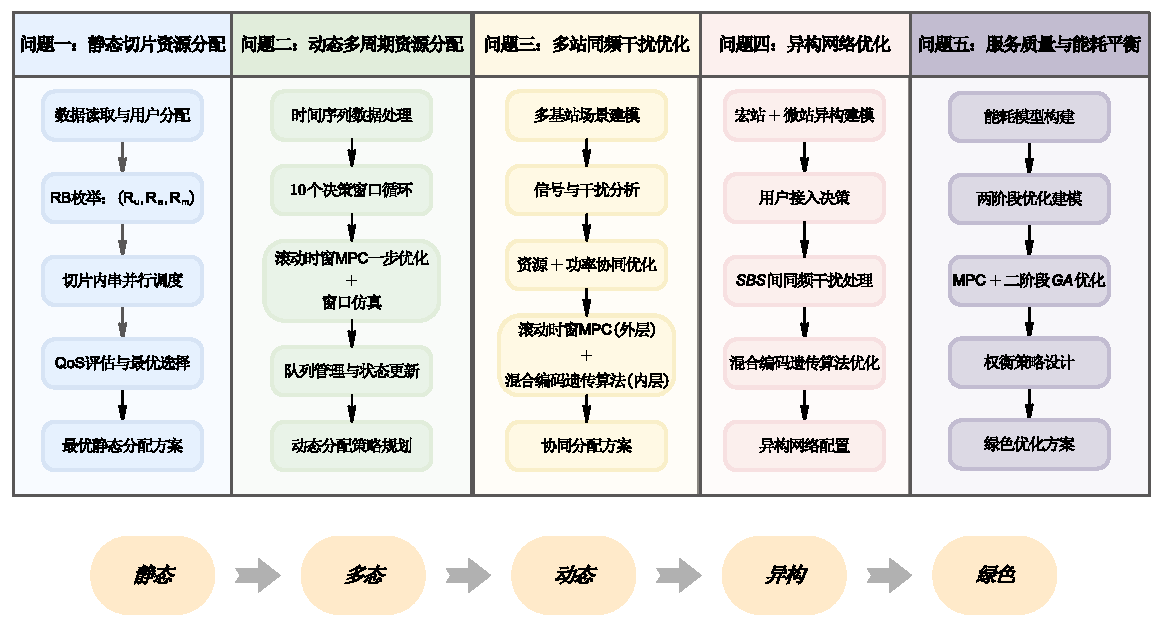
\includegraphics[width=1\textwidth]{figures/我们的工作.pdf}
    \caption{本文的主要工作流程与创新点概览}
    \label{fig:our_work}
\end{figure}

%%%%%%%%%%%%%%%%%%%%%%%%%%%%%%%%%%%%%%%%%%%%%%%%%%%%%%%%%%%%% 

\section{模型假设}
为简化问题,本文做出以下假设:

(1)假设所有资源分配决策在每个100ms决策窗口的开始时刻一次性做出,并在此窗口持续时间内保持不变。

    此假设使复杂的动态问题进行了简化,避免了因过于频繁的决策而导致的系统信令开销过大和优化问题难以求解的问题。

(2)假设一个基站的所有资源块全部划分,在用户在每种切片内部占用时可以浪费。

    此假设简化了求解结果,减少了资源分配的复杂性,在用户任务量较少时,分配的资源块可能并未使用,若不完全分配,会导致多种最优解,但实际上对应相同情形。

(3)假设eMBB切片的服务质量(QoS)中传输速率的计算在一次任务的传输中取平均速率。

    此假设简化了求解过程,避免了因传输速率计算复杂度高而导致的求解困难。
    

%%%%%%%%%%%%%%%%%%%%%%%%%%%%%%%%%%%%%%%%%%%%%%%%%%%%%%%%%%%%% 
\section{符号说明}
\begin{table}[H]
\centering
\rowcolors{2}{white}{blue!5}
\begin{tabularx}{1\textwidth}{c C c}
\toprule
\textbf{符号} & \textbf{含义} & \textbf{单位} \\
\midrule
$R_n$ & 基站$n$的RB总数(MBS:$100$;SBS:$50$) & RB \\
$b$ & 单个RB带宽($360$ kHz) & kHz \\
$v_s$ & 切片$s$内每用户占用的RB数(U/e/m为$10/5/2$) & RB \\
$x_{n,s}(t)$ & 基站$n$在窗口$t$为切片$s$分配的RB数 & RB \\
$p_{n,s}(t)$ & 基站$n$在窗口$t$对切片$s$的发射功率 & dBm \\
$\gamma_k(\tau)$ & 用户$k$在时刻$\tau$的信干噪比(SINR) & - \\
$r_k(\tau)$ & 用户$k$在时刻$\tau$的传输速率 & bps \\
$D_k$ & 用户$k$的任务数据量 & Mbit \\
$L_k^{s}$ & 用户$k$在切片$s$的总时延 & s \\
$Q_k(t)$ & 用户$k$在时刻$t$的队列积压量 & Mbit \\
$L_s^{\text{SLA}}$ & 切片$s$的时延SLA要求 & ms \\
$M_s$ & 切片$s$的任务丢失惩罚系数($s\in\{U,e,m\}$) & - \\
$E_{total}(t)$ & 窗口$t$内全网总能耗 & J \\
\bottomrule
\multicolumn{3}{r}{\footnotesize 注:未列出的以及重复的符号均以首次出现处为准。} \\
\end{tabularx}
\end{table}



%%%%%%%%%%%%%%%%%%%%%%%%%%%%%%%%%%%%%%%%%%%%%%%%%%%%%%%%%%%%% 
\section{问题一的模型的建立和求解}
\subsection{问题一的描述与分析}

问题一考虑单个微基站的资源分配场景。该基站拥有50个资源块(Resource Block, RB),需要为三类网络切片——URLLC(高可靠低时延)、eMBB(增强移动宽带)和mMTC(大规模机器通信)进行资源分配,以最大化用户服务质量。这是一个静态资源分配优化问题,需要在满足资源约束的条件下,找到最优的资源块分配方案。

\subsection{预备工作}
\subsubsection{关键参数补充}

\textbf{基站与信号参数}:基站发射功率 $p_{\text{tx}} = 30$ dBm,单个资源块(RB)带宽 $b = 360$ kHz,噪声系数 $NF = 7$ dB。

\textbf{决策周期}:系统每 $T_{\text{window}} = 100$ ms进行一次资源分配决策。

\textbf{切片资源占用与服务等级协议(SLA)}:URLLC切片:每个用户占用10个资源块,要求时延 $L_k^U \leq 5$ ms,速率 $r_k \geq 10$ Mbps;
eMBB切片:每个用户占用5个资源块,要求时延 $L_k^e \leq 100$ ms 且传输速率 $r_k \geq 50$ Mbps;
mMTC切片:每个用户占用2个资源块,要求时延 $L_k^m \leq 500$ ms,速率 $r_k \geq 1$ Mbps。


\textbf{QoS评估参数}:U切片的效益折扣系数 $\alpha = 0.95$,任务丢失惩罚 $M_U = 5$;e切片的任务丢失惩罚 $M_e = 3$;m切片的任务丢失惩罚 $M_m = 1$。



\subsection{模型建立}

\subsubsection{传输速率计算}

根据附录中的信号传输模型,用户$k$获得$i_k$个资源块时的接收功率为:

\begin{equation}
p_{\text{rx},k} = 10^{\frac{p_{\text{tx}} - \phi_k}{10}} \cdot |h_k|^2 \quad \text{(mW)}
\end{equation}
其中,$p_{\text{tx}}$为基站发射功率(dBm),$\phi_k$为大规模衰减(dB),$h_k$为小规模瑞利衰落系数,$p_{\text{rx},k}$为接收功率(mW)。

考虑噪声功率的影响,噪声功率谱密度为:

\begin{equation}
N_0 = -174 + 10\log_{10}(i_k \cdot b) + 7 \quad \text{(dBm)}
\end{equation}
其中,$i_k$为用户$k$占用的RB数量,$b$为单RB带宽(Hz),$-174$ dBm/Hz为热噪声谱密度,$7$ dB为噪声系数。

信干噪比(SINR)在无干扰情况下简化为信噪比(SNR):

\begin{equation}
\gamma_k = \frac{p_{\text{rx},k}}{10^{\frac{N_0}{10}}}
\end{equation}
其中,$N_0$以dBm计,$10^{\frac{N_0}{10}}$为噪声功率(mW)。

根据香农公式,用户$k$的传输速率为:

\begin{equation}
r_k = i_k \cdot b \cdot \log_2(1 + \gamma_k) \quad \text{(bps)}
\end{equation}
其中,$r_k$为传输速率(bps),$i_k$为RB数量,$b$为单RB带宽。

\subsubsection{时延计算模型}
根据附录中描述的用户任务服务流程,用户的总时延由排队时延和传输时延两部分构成。

用户$k$的传输时延$T_k$为完成其任务数据量$D_k$所需的传输时间,计算公式为:
\begin{equation}
T_k = \frac{D_k \times 10^6}{r_k} \quad \text{(s)}
\end{equation}
其中,$D_k$为任务数据量(Mbit),$r_k$为用户的传输速率(bps)。

用户的总时延$L_k^s$为排队时延$Q_k$与传输时延$T_k$之和:
\begin{equation}
L_k^{s} = Q_k + T_k, \quad s \in \{U, e, m\}
\end{equation}
其中,$Q_k$是在调度过程中产生的等待时间。

\subsubsection{服务质量评估函数}

根据附录中的用户服务质量定义,并结合计算出的总时延,不同切片的QoS评估函数如下:

\textbf{(1) U切片(URLLC)}

服务质量函数为:
\begin{equation}
y_k^{U} = \begin{cases}
\alpha^{L_k^{U}} & \text{若 } L_k^{U} \leq L_{U}^{\text{SLA}} \\
-M_{U} & \text{若 } L_k^{U} > L_{U}^{\text{SLA}}
\end{cases}
\end{equation}
其中,$\alpha\in(0,1)$为效益折扣系数(本题取$\alpha=0.95$),$M_U$为U切片任务丢失惩罚系数,$L_U^{\text{SLA}}$为U切片时延SLA。

\textbf{(2) e切片(eMBB)}

e切片用户采用三段式QoS函数:
\begin{equation}
y_k^{e} = \begin{cases}
1 & \text{若 } r_k \geq r_{e}^{\text{SLA}} \text{ 且 } L_k^{e} \leq L_{e}^{\text{SLA}} \\
\frac{r_k}{r_{e}^{\text{SLA}}} & \text{若 } r_k < r_{e}^{\text{SLA}} \text{ 且 } L_k^{e} \leq L_{e}^{\text{SLA}} \\
-M_{e} & \text{若 } L_k^{e} > L_{e}^{\text{SLA}}
\end{cases}
\end{equation}
其中,$r_e^{\text{SLA}}$、$L_e^{\text{SLA}}$分别为e切片的速率与时延SLA,$M_e$为惩罚系数。

\textbf{(3) m切片(mMTC)}

m切片的QoS基于接入成功率(满足时延SLA时按接入比例计分):
\begin{equation}
y_k^{m} = \begin{cases}
\frac{\sum_{i \in \mathcal{U}_{m}} c_i'}{\sum_{i \in \mathcal{U}_{m}} c_i} & \text{若 } L_k^{m} \le L_{m}^{\text{SLA}} \\
-M_{m} & \text{若 } L_k^{m} > L_{m}^{\text{SLA}}
\end{cases}
\end{equation}
其中,$\mathcal{U}_m$为m切片用户集合,$c_i$表示是否有任务需求,$c_i'$表示是否成功接入,$L_k^{m}$为用户$k$的总时延(同上定义),$M_m$为惩罚系数。

\subsubsection{优化模型}

基于上述分析,建立如下优化模型:

\begin{equation}
\begin{aligned}
\max_{n_U, n_e, n_m} \quad & Q = \sum_{s \in \mathcal{S}} \sum_{k \in \mathcal{U}_s} y_k^s \\
\text{s.t.} \quad & \begin{cases}
 n_U + n_e + n_m \leq N \\
 n_s \geq 0, \quad \forall s \in \mathcal{S} \\
 n_s \in \mathbb{Z}, \quad \forall s \in \mathcal{S}
 \end{cases}
 \end{aligned}
 \end{equation}
其中,$n_U, n_e, n_m$分别为分配给U、e、m切片的RB个数,$\mathcal{S}=\{U,e,m\}$,$\mathcal{U}_s$为切片$s$的用户集合;$y_k^{U}$、$y_k^{e}$为用户级QoS得分,$y^{m}$为m切片的聚合式接入比例得分。

其中,第一个约束为资源块总数限制,第二个约束为非负约束,第三个约束为整数约束。
\subsection{模型求解}

该优化问题属于整数规划问题,考虑到总资源块数量有限($N=50$),且各切片用户占用RB数量固定,使得分配给各切片的RB数量 $n_s$ 的可行组合是有限的。因此,我们采用枚举法结合调度仿真的策略进行求解,以确保找到全局最优解。算法流程如下:

\textbf{Step1:生成RB分配方案}

我们枚举所有满足约束条件的RB分配方案 $(n_U, n_e, n_m)$。为避免资源浪费,分配给各切片的RB数量应为其用户占用量的整数倍。具体地:
\begin{itemize}
    \item $n_U$ 在 $\{0, 10, 20, \dots, 50\}$ 中取值。
    \item $n_e$ 在 $\{0, 5, 10, \dots, 50 - n_U\}$ 中取值。
    \item $n_m = 50 - n_U - n_e$,并检验 $n_m$ 是否为2的倍数。若否则舍弃该方案。
\end{itemize}

\textbf{Step2:切片内调度与性能计算}

对于每一个有效的RB分配方案,我们在各切片内部独立进行调度仿真,以计算每个用户的性能指标。
\begin{itemize}
    \item \textbf{并发容量计算}:对于切片 $s \in \{U, e, m\}$,其并发服务能力为 $C_s = \lfloor n_s / v_s \rfloor$。
    \item \textbf{串并行调度}:在100ms决策周期内,我们采用一种串并行的服务策略。初始时,将前 $C_s$ 个用户(按用户编号排序)分配至并发信道进行传输。当某个用户完成传输后,其占用的信道立即释放,并分配给队列中的下一个用户。
    \item \textbf{性能计算}:通过该调度过程,我们可以计算出每个用户 $k$ 的传输时延 $T_k$ 和等待时延 $Q_k$,从而得到总时延 $L_k = Q_k + T_k$。用户的传输速率 $r_k$ 也一并计算得出。
\end{itemize}

\textbf{Step3:服务质量评估}

根据步骤2计算出的性能指标 $(L_k, r_k)$,我们依据模型中定义的服务质量评估函数计算每个用户的QoS得分 $y_k^s$,并汇总得到当前RB分配方案下的总服务质量 $Q = \sum y_k^s$。

\textbf{Step4:寻找最优方案}

遍历所有RB分配方案后,总服务质量 $Q$ 最高的方案即为问题的最优解。我们记录下最优方案对应的 $(n_U, n_e, n_m)$ 组合、各用户的详细性能指标以及最终的总QoS值。

\subsection{求解结果}
通过执行上述算法,我们得到的最优资源分配方案及对应的性能指标如下:

\textbf{最优资源分配方案}

经枚举计算,我们找到了3个并列的最优资源分配方案,它们均能使系统总服务质量达到最大值15.7823。这三个方案的具体RB分配如下表所示。

\begin{table}[H]
\centering
\caption{并列最优资源分配方案}
\label{tab:q1_best_solutions}
\begin{tabular}{cccccc}
\hline
\textbf{方案} & \textbf{URLLC RB数 ($n_U$)} & \textbf{eMBB RB数 ($n_e$)} & \textbf{mMTC RB数 ($n_m$)} & \textbf{总QoS} \\
\hline
1 & 20 & 10 & 20 & 15.7823 \\
2 & 20 & 20 & 10 & 15.7823 \\
3 & 30 & 10 & 10 & 15.7823 \\
\hline
\end{tabular}
\end{table}

在以上所有方案中,各切片获得的QoS合计分数均相同,分别为:URLLC QoS合计1.9870,eMBB QoS合计3.7953,mMTC QoS合计10.0000。

\textbf{结果分析}

\begin{itemize}
    \item \textbf{最优性分析}:计算结果显示,存在三个不同的RB分配方案能够达到相同的最优目标函数值15.7823,如上表\ref{tab:q1_best_solutions}所示。这些方案的共同点在于,它们为URLLC、eMBB和mMTC切片带来的QoS贡献是完全相同的。这表明在当前用户任务和信道条件下,只要分配给U切片、eMBB切片和mMTC切片的RB数量分别不低于20、10和10个,就能保证所有用户达到最佳的服务水平。这种现象说明资源配置具有一定的灵活性和鲁棒性。
    \item \textbf{用户性能详情}:在任何一个最优方案下,各用户的性能指标均相同。所有URLLC用户的时延均远低于5ms的SLA要求(如U1为0.145ms,U2为0.110ms),QoS得分接近1。eMBB用户中,e1, e2, e4满足速率与时延双重标准,QoS为1;e3用户速率未达标(39.77 Mbps < 50 Mbps),但仍在SLA时延内,获得了比例得分0.7953。所有mMTC用户均在极低时延下完成传输(均小于1ms),远优于500ms的SLA标准,因此获得了满分。
    \item \textbf{资源效率与选择}:这三个方案均实现了资源的高效利用。在实际部署中,可以根据网络运营商的偏好进行选择。例如,方案1(20, 10, 20)为mMTC分配了最多的资源,适合未来mMTC连接数可能增加的场景;方案2(20, 20, 10)则向eMBB倾斜,适合视频流量大的场景;方案3(30, 10, 10)则最优先保障URLLC业务。这些方案共同构成了问题的最优解集。
\end{itemize}

综上所述,我们提出的资源分配方案能够有效满足各类切片用户的服务需求,实现了系统整体服务质量的最优。
\section{问题二的模型的建立和求解}
\subsection{问题二的描述与分析}

问题二考虑动态环境下的多时间段资源分配场景。与问题一的静态单时刻分配不同,问题二面临用户移动性、信道时变性以及任务队列动态变化的复杂问题。在1000ms的观测窗口内,系统需要每100ms进行一次资源分配决策(共10次),既要处理新到达的任务,又要考虑积压在排队队列中的历史任务。这是一个多阶段动态优化问题,需要在时间维度上综合考虑任务到达、信道变化和排队延迟的耦合影响。

\subsection{预备工作}

\subsection{模型建立}

问题二模型大部分与问题一相同,不同之处在于问题二允许 $t$ 在决策窗口内按 $\mathcal{T}=\{0,100,\dots,900\}$ 演化,并引入任务到达与队列动态。为避免重复,问题二中与问题一中相同的定义与公式不再赘述。

\subsubsection{任务队列动态演化模型}

为精确描述任务的动态变化,我们引入两个时间尺度:
\begin{itemize}
    \item \textbf{决策时刻 $t$}:每100ms进行一次资源分配决策,对应$t \in \{0, 100, 200, \ldots, 900\}$。
    \item \textbf{仿真时刻 $\tau$}:以1ms为步长,用于模拟任务到达和信道变化,$\tau$表示具体的毫秒时刻。
\end{itemize}

定义用户$k$在时刻$t$的任务队列状态:

\begin{itemize}
  \item $A_{k,\tau}(t)$:用户$k$在时刻$\tau$到达且在时刻$t$仍在队列中的任务数据量(Mbit)
  \item $Q_k(t) = \sum_{\tau=0}^{t} A_{k,\tau}(t)$:用户$k$在时刻$t$的总排队任务量
  \item $W_k(t)$:用户$k$在时刻$t$已等待的排队时间
\end{itemize}

任务队列的动态演化遵循以下规律:

\textbf{(1) 任务到达:}
在每个1ms时刻$\tau$,根据数据文件读取新到达任务:
\begin{equation}
A_{k,\tau}(\tau) = \text{TaskFlow}_k(\tau)
\end{equation}

\textbf{(2) 任务服务:}
在决策时刻$t$,若用户$k$被分配$i_k(t)$个RB,则在接下来的100ms内可传输的数据量为:
\begin{equation}
S_k(t) = r_k(t) \times 0.1 \times 10^{-6} \quad \text{(Mbit)}
\end{equation}

\textbf{(3) 队列更新:}
任务按FIFO顺序服务,队列更新规则为:
\begin{equation}
\label{eq:queue_evolution}
Q_k(t+100) = \max\left(0, Q_k(t) + \sum_{\tau=t+1}^{t+100} \text{TaskFlow}_k(\tau) - S_k(t)\right)
\end{equation}

\subsubsection{时延计算模型(任务级)}
 
由于存在到达过程,问题二按任务到达时刻进行时延度量。对于用户$k$在时刻$\tau$到达的任务,其总时延包含排队时延和传输时延:

\textbf{(1) 排队时延:}
任务在时刻$\tau$到达,在时刻$t_{\text{start}}$开始服务,则排队时延为:
\begin{equation}
Q_{k,\tau} = t_{\text{start}} - \tau
\end{equation}

\textbf{(2) 传输时延:}
假设任务从时刻$t_{\text{start}}$开始传输,数据量为$D_{k,\tau}$,则传输时延为:
\begin{equation}
T_{k,\tau} = \frac{D_{k,\tau} \times 10^6}{r_k(t_{\text{start}})}
\end{equation}

\textbf{(3) 总时延:}
\begin{equation}
L_{k,\tau}^s = Q_{k,\tau} + T_{k,\tau}, \quad s \in \{U, e, m\}
\end{equation}

\subsubsection{动态服务质量评估函数}
 
在多时间段场景下,各切片的QoS评估在问题一基础上作如下时间聚合:

\textbf{(1) URLLC切片:}
对于在时间窗口$[0, 1000]$ms内完成的所有URLLC任务:
\begin{equation}
y_{k,\tau}^{U} = \begin{cases}
\alpha^{L_{k,\tau}^{U}} & \text{若 } L_{k,\tau}^{U} \leq L_{U}^{\text{SLA}} \\
-M_{U} & \text{若 } L_{k,\tau}^{U} > L_{U}^{\text{SLA}}
\end{cases}
\end{equation}

\textbf{(2) eMBB切片:}
对于在决策时刻$t$服务的eMBB用户$k$:
\begin{equation}
y_{k}^{e}(t) = \begin{cases}
1 & \text{若 } r_k(t) \geq r_{e}^{\text{SLA}} \text{ 且 } L_{k,\tau}^{e} \leq L_{e}^{\text{SLA}} \\
\frac{r_k(t)}{r_{e}^{\text{SLA}}} & \text{若 } r_k(t) < r_{e}^{\text{SLA}} \text{ 且 } L_{k,\tau}^{e} \leq L_{e}^{\text{SLA}} \\
-M_{e} & \text{若} L_{k,\tau}^{e} > L_{e}^{\text{SLA}}
\end{cases}
\end{equation}

\textbf{(3) mMTC切片:}
在每个决策时刻$t$,对每个mMTC用户$k$的QoS评估为:
\begin{equation}
y_k^{m}(t) = \begin{cases}
\dfrac{\sum_{i \in \mathcal{U}_{m}} c_i'(t)}{\sum_{i \in \mathcal{U}_{m}} c_i(t)} & \text{若 } L_k^{m}(t) \le L_{m}^{\text{SLA}} \\
-M_{m} & \text{若 } L_k^{m}(t) > L_{m}^{\text{SLA}}
\end{cases}
\end{equation}
其中,$c_i(t)$表示用户$i$在时刻$t$是否有待服务任务,$c_i'(t)$表示是否成功接入服务。

\subsubsection{多时间段优化模型}
 
基于上述分析,建立如下多时间段动态优化模型(目标在整个时间窗口跨$t$求和):

\begin{equation}
\begin{aligned}
\max_{\{n_s(t)\}_{s,t}} \quad & Q_{\text{total}} = \sum_{t \in \mathcal{T}} \left[ \sum_{k \in \mathcal{U}_U} y_{k}^{U}(t) + \sum_{k \in \mathcal{U}_e} y_{k}^{e}(t) + \sum_{k \in \mathcal{U}_m} y_{k}^{m}(t) \right]\\
\text{s.t.} \quad & \begin{cases}
 n_U(t) + n_e(t) + n_m(t) = 50\\
 n_U(t) \bmod 10 = 0,\; n_e(t) \bmod 5 = 0,\; n_m(t) \bmod 2 = 0\\
 Q_k(t+100) = \max\!\left(0, Q_k(t) + \Delta A_k(t) - S_k(t)\right) \\
 n_s(t) \in \mathbb{Z}_{\ge 0}\\
 \forall t \in \mathcal{T},\; \forall k,\; \forall s \in \mathcal{S}
 \end{cases}
 \end{aligned}
 \end{equation}
其中,$\mathcal{T} = \{0, 100, 200, \ldots, 900\}$为决策时刻集合,$n_s(t)$为时刻$t$分配给切片$s$的RB数量,$Q_k(t)$为用户$k$在时刻$t$的排队任务量,$\Delta A_k(t)$为时间段$[t, t+100)$内用户$k$的新增任务量。

该模型的核心挑战在于:(1) 状态空间的指数级增长;(2) 任务到达的随机性与信道的时变性;(3) 排队时延与传输时延的耦合优化。需要设计高效的求解算法来处理这一复杂的多阶段随机优化问题。

\subsection{模型求解}

问题二是一个多阶段动态优化问题。由于状态空间(用户队列、信道状况)随时间演化,且任务到达具有随机性,精确求解该问题通常需要复杂的动态规划或强化学习方法,计算成本极高。考虑到决策周期较短,且需要快速响应,我们采用一种基于模型预测控制(Model Predictive Control, MPC)思想的贪心策略(Myopic Policy),也称为“单步前瞻优化”。该策略在每个决策窗口的起点,仅优化当前窗口的性能,而不考虑对未来窗口的长期影响。这种方法在实践中被证明是有效且计算可行的。

算法的核心思想是:在每个决策时刻 $t \in \{0, 100, \dots, 900\}$,我们面对当前的系统状态(主要是各用户的任务队列),通过枚举所有可能的RB分配方案,并对每种方案进行精细化的仿真,来预测未来100ms内的系统服务质量。然后,我们选择能使当前窗口QoS最大化的方案进行实施,并将演化后的系统状态作为下一个决策时刻的初始条件。具体算法流程如下:

\textbf{Step1:初始化}

在仿真开始时刻 $t=0$,初始化所有用户的任务队列为空。

\textbf{Step2:逐窗口迭代决策}

对于每个决策窗口 $w$(对应时间段 $[t, t+100)$,其中 $t = w \times 100$):

\begin{enumerate}
    \item \textbf{生成RB分配方案}:与问题一类似,我们首先枚举所有满足约束条件的RB分配方案 $(n_U(t), n_e(t), n_m(t))$。确保资源总量为50,且每个切片的RB数量满足其最小占用粒度(URLLC为10的倍数,eMBB为5的倍数,mMTC为2的倍数)。

    \item \textbf{窗口内调度仿真与评估}:对于每一个生成的RB分配方案,我们执行一次为期100ms的详细仿真,以评估其性能。
    \begin{itemize}
        \item \textbf{初始状态}:仿真从当前决策时刻 $t$ 的系统状态开始,包括所有用户当前的排队任务。
        \item \textbf{动态演化}:在100ms的仿真窗口内,我们以1ms为步长进行演化:
        \begin{itemize}
            \item \textbf{任务到达}:根据附件二的数据,在每个1ms时刻,将新到达的任务加入对应用户的队列。
            \item \textbf{调度与服务}:根据当前切片的并发容量 $C_s = \lfloor n_s(t) / v_s \rfloor$,采用“编号靠前优先”的原则,为有任务排队的用户分配服务信道。正在服务的用户将根据其在当前ms的信道质量计算出的速率来处理任务。
            \item \textbf{资源释放与接续}:当一个用户的任务完成时,其占用的并发槽位被立即释放。调度器会立刻检查该切片内是否有其他排队的用户(同样按编号顺序),若有则立即接续服务。
        \end{itemize}
        \item \textbf{性能计算}:在仿真过程中,我们精确记录每个任务的到达、开始服务和完成的时刻,从而计算其端到端时延。对于在当前100ms窗口内完成的每一个任务,我们根据其所属切片的服务质量评估函数计算QoS得分。
    \end{itemize}
    
    \item \textbf{选择最优方案并更新状态}:遍历所有RB分配方案后,我们选择在当前窗口内获得累计QoS总分最高的方案作为本次决策的结果。然后,我们将该最优方案对应的仿真结束时刻($t+100$)的用户队列状态,作为下一个决策窗口的初始状态。
\end{enumerate}

\textbf{Step3:汇总结果}

重复Step2,直到完成所有10个决策窗口($t=0$至$t=900$)的决策。最后,将每个窗口获得的最优QoS得分进行累加,得到整个1000ms内的总服务质量。通过这种方式,我们得到了一系列动态的RB分配决策,以及最终的系统整体性能评估。

\subsection{求解结果}

通过执行上述基于MPC的贪心算法,我们得到了1000ms内的动态资源分配策略,其总服务质量达到了\textbf{352.1029}。

\subsubsection{最优资源分配序列}

算法在10个决策窗口中选择的RB分配序列如下表所示。该序列是在每个窗口选择瞬时最优解(若有多个则选择第一个)的结果。

\begin{table}[H]
\centering
\caption{问题二动态资源分配序列}
\label{tab:q2_decision_sequence}
\begin{tabular}{ccccc}
\hline
\textbf{决策时刻 (ms)} & \textbf{URLLC RB数 ($n_U$)} & \textbf{eMBB RB数 ($n_e$)} & \textbf{mMTC RB数 ($n_m$)} & \textbf{窗口QoS} \\
\hline
0 & 10 & 20 & 20 & 65.490 \\
100 & 10 & 20 & 20 & 40.028 \\
200 & 10 & 20 & 20 & 38.835 \\
300 & 10 & 0 & 40 & 32.800 \\
400 & 20 & 0 & 30 & 31.850 \\
500 & 10 & 0 & 40 & 24.250 \\
600 & 10 & 0 & 40 & 27.100 \\
700 & 20 & 0 & 30 & 32.800 \\
800 & 20 & 0 & 30 & 31.850 \\
900 & 20 & 0 & 30 & 27.100 \\
\hline
\textbf{总计} & - & - & - & \textbf{352.103} \\
\hline
\end{tabular}
\end{table}

在整个仿真周期内,各切片累计获得的QoS分数分别为:URLLC QoS合计\textbf{205.8175},eMBB QoS合计\textbf{46.2854},mMTC QoS合计\textbf{100.0000}。

\subsubsection{并列最优解分析}

值得注意的是,在多个决策窗口中,算法发现了多个能够达到相同最优QoS的RB分配方案。这为网络运营商提供了在满足性能目标的同时,根据其他策略(如能耗、资源均衡等)进行选择的灵活性。下表列出了部分存在并列最优解的决策时刻及其方案。

\begin{table}[H]
\centering
\caption{部分决策窗口的并列最优方案}
\label{tab:q2_tie_solutions}
\begin{tabular}{ccc}
\hline
\textbf{决策时刻 (ms)} & \textbf{窗口最优QoS} & \textbf{并列最优RB分配方案 ($n_U, n_e, n_m$)} \\
\hline
\multirow{3}{*}{300} & \multirow{3}{*}{32.800} & (10, 0, 40) \\
 & & (20, 0, 30) \\
 & & (30, 0, 20) \\
\hline
\multirow{3}{*}{400} & \multirow{3}{*}{31.850} & (20, 0, 30) \\
 & & (30, 0, 20) \\
 & & (40, 0, 10) \\
\hline
\multirow{3}{*}{600} & \multirow{3}{*}{27.100} & (10, 0, 40) \\
 & & (20, 0, 30) \\
 & & (30, 0, 20) \\
\hline
\multirow{2}{*}{900} & \multirow{2}{*}{27.100} & (20, 0, 30) \\
 & & (30, 0, 20) \\
\hline
\end{tabular}
\end{table}

\subsubsection{结果分析}

\begin{itemize}
    \item \textbf{动态适应性}:从资源分配序列(表 \ref{tab:q2_decision_sequence})可以看出,算法展现了良好的动态适应性。在仿真初期(0-300ms),eMBB业务有大量任务到达,算法明智地为其分配了20个RB以快速处理,获得了较高的QoS。在300ms后,eMBB任务队列清空,算法果断地将其RB资源完全回收,转而分配给URLLC和mMTC,以应对后续的URLLC任务并保证mMTC的稳定接入。
    \item \textbf{资源分配的灵活性}:如表 \ref{tab:q2_tie_solutions} 所示,从300ms开始,系统中出现了大量的并列最优解。这些方案的共同点是都放弃了为eMBB分配资源(因为其队列已空),而将资源在URLLC和mMTC之间进行权衡。例如在300ms时,(10, 0, 40), (20, 0, 30), (30, 0, 20)三种方案都能达到相同的最优QoS。这表明在满足核心性能指标后,资源配置具有相当的灵活性。运营商可以根据长期策略选择更偏向URLLC(保障未来可能的高优先级任务)或更偏向mMTC(扩大连接容量)的方案。
    \item \textbf{切片性能分析}:URLLC切片的所有任务均在远低于SLA(5ms)的时延内完成,获得了很高的QoS分数。eMBB切片在前期获得了足够的资源,其QoS贡献主要来自前300ms。mMTC切片由于其“尽力而为”和高并发的特性,在整个周期内稳定地获得了满分的QoS。这说明我们采用的MPC贪心策略成功地平衡了三类业务的需求。
\end{itemize}

综上所述,我们提出的动态资源分配模型与求解算法,能够在时变的信道和任务到达条件下,做出快速有效的决策,实现了系统在整个时间窗口内总服务质量的最优。
\section{问题三的模型的建立和求解}
\subsection{问题三的描述与分析}

\subsection{预备工作}


\subsubsection{集合、索引与参数}

为适配附件三的多微基站、同频复用且存在小区间干扰的场景,定义如下集合与索引:

\begin{itemize}
  \item 基站集合:$\mathcal{N}=\{1,2,3\}$(分别对应 BS1、BS2、BS3)。
  \item 切片集合:$\mathcal{S}=\{U,e,m\}$,分别对应 URLLC、eMBB、mMTC。
  \item 用户集合:$\mathcal{K}=\mathcal{K}_U\cup\mathcal{K}_e\cup\mathcal{K}_m$,其中 $\mathcal{K}_U=\{\mathrm{U1},\mathrm{U2}\}$,$\mathcal{K}_e=\{\mathrm{e1},\dots,\mathrm{e12}\}$,$\mathcal{K}_m=\{\mathrm{m1},\dots,\mathrm{m30}\}$。
  \item 决策时刻集合:$\mathcal{T}=\{0,100,\dots,900\}$(单位 ms),每个决策窗口长度为 $100$ ms;窗口内以 $1$ ms 步长进行链路与队列仿真,记窗口内细粒度时刻集合为 $\mathcal{F}(t)=\{t,t+1,\dots,t+99\}$。
\end{itemize}

关键系统参数(与问题一、二保持一致):

\begin{itemize}
  \item 每站可用 RB 总数 $R_{\text{tot}}=50$;单 RB 带宽 $b=360\,\mathrm{kHz}$;噪声系数 $NF=7\,\mathrm{dB}$;
  \item 切片占用粒度:$i_U=10,\ i_e=5,\ i_m=2$(每个并发用户占用的 RB 数);
  \item 发射功率决策范围(第三问):$p_{n,s}(t)\in[10,30]\,\mathrm{dBm}$,为“基站 $n$ 在窗口 $t$ 对切片 $s$ 的统一每 RB 功率”(切片内各 RB 功率一致)。
\end{itemize}

\subsection{模型建立}

\subsubsection{信道与干扰模型}

附件三提供了每 $1$ ms 的大规模损耗 $\phi_{n,k}(\tau)$(dB)与小规模瑞利衰落 $h_{n,k}(\tau)$。设窗口 $t\in\mathcal{T}$ 内细粒度时刻为 $\tau\in\mathcal{F}(t)$,若用户 $k\in\mathcal{K}_s$ 在窗口 $t$ 由基站 $n$ 服务且被分配切片 $s$ 的 RB,则其接收功率(mW)为
\begin{equation}
 p_{\mathrm{rx},n\to k}(\tau)=10^{\frac{p_{n,s}(t)-\phi_{n,k}(\tau)}{10}}\cdot |h_{n,k}(\tau)|^2.
\end{equation}

噪声功率与占用 RB 数 $i$ 成正比,换算为线性功率(mW):
\begin{equation}
 N_0(i)=10^{\frac{-174+10\log_{10}(i\cdot b)+NF-30}{10}}.
\end{equation}

微基站同频复用引入同信道干扰。为保持“同一 RB 索引才互扰”的规则,我们令每站在窗口 $t$ 内将其 $50$ 个 RB 在频域上按切片连续划分且次序固定(例如 U-e-m),每个切片获得一段连续 RB 区间,跨站的相同 RB 索引构成同信道。于是用户 $k$ 的瞬时信干噪比为
\begin{equation}
 \gamma_k(\tau)=\frac{p_{\mathrm{rx},n\to k}(\tau)}{\sum\limits_{u\in\mathcal{N},\ u\neq n} I_{u\to k}(\tau)+N_0(i_s)},\quad s\in\mathcal{S},
\end{equation}
其中 $I_{u\to k}(\tau)$ 表示来自他站 $u$、在与 $k$ 所占 RB 索引重叠的切片 RB 上的干扰功率,按与上式相同的接收功率表达(由 $p_{u,s'}(t),\phi_{u,k}(\tau),h_{u,k}(\tau)$ 决定)。基于香农公式,窗口内瞬时速率为
\begin{equation}
 r_k(\tau)=i_s\cdot b\cdot \log_2\big(1+\gamma_k(\tau)\big)\quad(\mathrm{bps}).
\end{equation}
\subsubsection{任务到达与队列演化}

任务队列的动态演化过程与问题二完全一致,队列状态 $Q_k(t)$ 仍以每个用户为中心进行追踪,其演化遵循公式 \eqref{eq:queue_evolution}。

关键区别在于,服务量 $S_k(t)$ 的计算变得更为复杂,因为它取决于用户 $k$ 在当前窗口 $t$ 接入了哪个基站 $n$,以及所有基站的功率决策 $\{p_{n,s}(t)\}$。这将在后续的服务质量评估函数中具体体现。


\subsubsection{RB 切片并发与调度规则}

令 $x_{n,s}(t)$ 为窗口 $t$ 时基站 $n$ 切片 $s$ 的 RB 数,满足 $\sum_{s\in\mathcal{S}}x_{n,s}(t)=R_{\text{tot}}$。切片 $s$ 的并发容量为
\begin{equation}
 C_{n,s}(t)=\big\lfloor x_{n,s}(t)/i_s\big\rfloor.
\end{equation}
窗口内采用“编号靠前优先”的串-并行调度:每个 $(n,s)$ 最多同时服务 $C_{n,s}(t)$ 个队头任务,任务完成即释放并补位。URLLC 在切片内可按紧迫度(距 SLA 的剩余时限)优先。

\subsubsection{QoS 评估函数}

服务质量(QoS)的评估与前几问一致,核心是衡量每个任务的时延和速率是否满足服务等级协议(SLA)。

首先,我们需要计算每个任务的总时延。对于一个在时刻 $\tau$ 到达、数据量为 $D_{k,\tau}$ 的任务,其总时延 $L^{s}_{k,\tau}$ 由排队时延和传输时延两部分构成:
\begin{equation}
    L^{s}_{k,\tau} = \underbrace{(t_{\text{start}} - \tau)}_{\text{排队时延}} + \underbrace{\frac{D_{k,\tau} \cdot 10^6}{\bar{r}_k(t_{\text{start}})}}_{\text{传输时延}}
\end{equation}
其中,$t_{\text{start}}$ 是该任务开始被服务的时刻,$\bar{r}_k(t_{\text{start}})$ 是服务期间的平均数据速率。

然后,基于计算出的时延和瞬时速率,我们采用与前文相同的任务级 QoS 函数 $y^{s}_{k,\tau}$:
\begin{align}
 y^{U}_{k,\tau} &= \begin{cases}
 \alpha^{L^{U}_{k,\tau}} & L^{U}_{k,\tau}\le L^{\text{SLA}}_{U}\\
 -M_U & \text{否则}
 \end{cases} \\
y^{e}_{k,\tau} &= \begin{cases}
 1 & r_{k}(\tau_\text{srv})\ge r^{\text{SLA}}_{e}\ \text{and}\ L^{e}_{k,\tau}\le L^{\text{SLA}}_{e}\\
 \dfrac{r_{k}(\tau_\text{srv})}{r^{\text{SLA}}_{e}} & r_{k}(\tau_\text{srv})< r^{\text{SLA}}_{e}\ \text{and}\ L^{e}_{k,\tau}\le L^{\text{SLA}}_{e}\\
 -M_e & \text{否则}
 \end{cases} \\
 y^{m}_{k,\tau} &= \begin{cases}
 \dfrac{\sum\limits_{i\in\mathcal{K}_m}c'_i}{\sum\limits_{i\in\mathcal{K}_m}c_i} & L^{\,m}_{k,\tau}\le L^{\text{SLA}}_{m}\\
 -M_m & \text{否则}
 \end{cases}
\end{align}
参考取值:$\alpha=0.95$,$r^{\text{SLA}}_e=50\,\mathrm{Mbps}$,$L^{\text{SLA}}_{U}=5\,\mathrm{ms}$,$L^{\text{SLA}}_{e}=100\,\mathrm{ms}$,$L^{\text{SLA}}_{m}=500\,\mathrm{ms}$,$M_U=5, M_e=3, M_m=1$。

\subsubsection{决策变量与优化模型}

决策变量:
\begin{itemize}
  \item RB 切片分配:$x_{n,s}(t)\in\mathbb{Z}_{\ge 0}$
  \item 发射功率:$p_{n,s}(t)\in[10,30]\,\mathrm{(dBm)}$
  \item 接入关联:$a_{n,k}(t)\in\{0,1\}$,当 $a_{n,k}(t)=1$ 则 $k$ 在窗口 $t$ 仅由站 $n$ 调度
\end{itemize}

综合上述要素,第三问的动态联合优化模型可表述为(跨 10 个窗口聚合):
\begin{equation}
\begin{aligned}
\max_{\{x,p,a\}}\quad & Q_{\text{total}}=\sum_{t\in\mathcal{T}}\Bigg[\sum_{k\in\mathcal{K}_U}\sum_{\tau\in\mathcal{A}_k(t)} y^{U}_{k,\tau}+\sum_{k\in\mathcal{K}_e}\sum_{\tau\in\mathcal{A}_k(t)} y^{e}_{k,\tau}+\sum_{k\in\mathcal{K}_m}\sum_{\tau\in\mathcal{A}_k(t)} y^{m}_{k,\tau}\Bigg] \\
\text{s.t.}\quad & 
\left\{
\begin{aligned}
&\sum_{s\in\mathcal{S}} x_{n,s}(t)=50 \\
&x_{n,U}(t)\bmod 10=0 ,x_{n,e}(t)\bmod 5=0 ,x_{n,m}(t)\bmod 2=0 \\
&x_{n,s}(t)\in\mathbb{Z}_{\ge 0} \\
&10\le p_{n,s}(t)\le 30\\
&Q_k(t+100)=\max\Big\{0,\ Q_k(t)+\sum_{\tau\in\mathcal{F}(t)} D_k(\tau)-S_k(t)\Big\} \\
&r_k(\tau),\ \gamma_k(\tau)\ \text{由}\ (x,p,a)\ \text{与}\ (\phi,h)\ \text{及调度生成} \\
&\sum_{n\in\mathcal{N}} a_{n,k}(t)\le 1 \\
&\forall n\in\mathcal{N},\ t\in\mathcal{T},\ \forall n,k,s,t
\end{aligned}
\right.
\end{aligned}
\end{equation}
其中 $\mathcal{A}_k(t)\subseteq\mathcal{F}(t)$ 为窗口 $t$ 内属于用户 $k$ 且在 SLA 内完成的任务到达时刻集合;$r_k(\tau)$ 与 $S_k(t)$ 均受干扰耦合与调度影响,是 $(x,p,a)$ 的非线性函数。\\
该模型体现了“多站同频干扰 + 切片化 RB 分配 + 切片级功率控制 + 任务队列”的耦合特性,属于带整数约束与非凸干扰项的时变 MINLP 问题。

\subsection{模型求解}

在前两问的“切片 RB 枚举 + 预测–控制 (MPC)”框架无法直接扩展到第三问的原因在于:
1) 决策维度急剧扩张,包含了 9 个连续的功率变量 $\{p_{n,s}\}$ 与 48 个离散的用户接入基站变量 $\{a_{n,k}\}$,构成了庞大的混合搜索空间。
2) 小区间干扰项使目标函数呈现强非凸、非线性特性,枚举或传统凸优化方法难以求解,计算量将呈指数级爆炸。

为兼顾求解质量与计算效率,本问采用“\textbf{滚动时窗预测控制(MPC)}+\textbf{混合编码遗传算法(GA)}”的两层求解范式。其总体求解流程如图~\ref{fig:flow_q3}所示。

\begin{figure}[htbp]
  \centering
  %\includesvg[width=0.95\textwidth]{q3_flowchart.svg}
  \caption{问题三“滚动 MPC + GA”求解流程图}
  \label{fig:flow_q3}
\end{figure}

\subsubsection{外层:滚动时窗预测控制 (MPC)}
我们将 1000 ms 的总时长离散为 10 个长度为 $T_w=100$ ms 的独立决策窗口。在每个窗口 $t$ 的开始,我们求解一个静态优化问题,以确定该窗口内恒定不变的资源分配策略(包括用户接入、RB切片、功率等级)。这种滚动优化的方式使得模型可以应对时变的信道和业务。

在我们的实现中,为降低问题的复杂度,我们做了一项简化:在每个窗口的优化求解阶段,我们假设该窗口开始时所有用户的任务队列均为空,即不考虑由前一个窗口积压下来的任务。优化过程仅针对当前窗口内新到达的任务负载。这使得每个窗口的优化问题可以解耦和独立求解。

\subsubsection{内层:混合编码遗传算法 (GA)}
针对每个窗口内的静态资源分配问题,我们设计了遗传算法进行启发式搜索。GA 能够有效处理高维、非凸、含混合变量的复杂优化问题。
\begin{itemize}
    \item \textbf{个体编码方案}:每个个体(染色体)代表一个完整的资源分配策略,采用混合编码,由三部分组成:
    \begin{enumerate}
        \item \textbf{用户接入决策}:长度为 48 的整数向量,每个基因位代表一个用户,其值(0, 1, 2)表示该用户接入的基站(BS1, BS2, BS3)。
        \item \textbf{RB 切片分配}:长度为 6 的整数向量,每两位表示一个基站为 URLLC 和 eMBB 切片分配的 RB 数量。mMTC 切片的比例则由剩余资源确定,并根据切片粒度约束进行解码。
        \item \textbf{切片功率控制}:长度为 9 的浮点数向量,每个基因位表示一个基站上特定切片(U/E/M)的发射功率(dBm),范围在 $[10, 30]$。
    \end{enumerate}
    \item \textbf{适应度函数}:个体的适应度由一个精细的仿真器评估。该仿真器将个体解码后的策略作为输入,以 1 ms 为步长模拟整个 100 ms 窗口的动态过程。仿真完整地计算了用户速率(包含所有基站的同频干扰)、任务队列的演化以及最终产生的 QoS 总分。该 QoS 总分即为个体的适应度。
    \item \textbf{遗传算子与参数}:
    GA 采用精英保留策略,并使用锦标赛选择、算术交叉(针对连续变量)/单点交叉(针对离散变量)和高斯/随机扰动变异(针对不同类型变量)来产生新一代种群。关键参数设置如下:种群大小为 40,最大进化代数为 200,精英个体保留 5 个,交叉概率 0.8,变异概率 0.3。
\end{itemize}

\subsubsection{求解流程}
算法的总体流程遵循“滚动时窗预测控制”框架,将1000ms的动态问题分解为10个独立的百毫秒优化窗口。在每个窗口的起点,我们利用遗传算法求解一个静态的资源分配优化问题。具体流程如下:

\textbf{Step 1:初始化}
在仿真开始前,通过 $`build_env`$函数一次性加载“附件三”中所有必需的数据,包括所有用户的任务到达流、各基站到各用户的大规模路径损耗和小规模瑞利衰落信道数据。

\textbf{Step 2:逐窗口迭代决策}
对于每个决策窗口 $w$(对应时间段 $[t, t+100)$,其中 $t = w \times 100$),执行以下内层优化:

\begin{enumerate}
    \item \textbf{GA种群初始化}:在窗口 $t$ 开始时,随机生成一个由 40 个个体组成的初始种群。每个个体(染色体)都代表了该窗口的一种完整资源分配方案,其编码包含了用户接入、RB切片和功率控制三部分决策。

    \item \textbf{适应度评估(窗口内仿真)}:对种群中的每一个个体,通过调用一个精细的仿真器$(`simulate_window_multibs`)$来评估其适应度(即QoS得分)。
    \begin{itemize}
        \item \textbf{空队列假设}:为使各窗口的优化问题解耦,仿真器在评估开始时,\textbf{假设所有用户的任务队列均为空}。它只考虑在当前$100ms$窗口内新到达的任务。
        \item \textbf{动态演化}:仿真器以1ms为步长,模拟100ms内的动态过程。在每个ms,它会处理新任务的到达,并根据个体所代表的资源分配方案(用户归属、RB和功率)以及全网的同频干扰,计算每个正在服务用户的瞬时速率,并更新其任务处理进度。
        \item \textbf{性能计算}:仿真器精确追踪每个任务从到达、排队到完成的完整生命周期,计算其端到端时延和平均速率,并依据QoS评估函数计算得分。所有在窗口内完成的任务的QoS得分总和,即为该个体的适应度。
    \end{itemize}

    \item \textbf{遗传进化}:采用精英保留策略,通过锦标赛选择、交叉和变异等遗传算子,从当前代种群生成下一代种群。此过程重复迭代 $200$ 代。

    \item \textbf{选择最优方案}:在$200$代进化完成后,选择整个过程中适应度最高的个体,将其解码为当前窗口 $w$ 的最终资源分配决策。
\end{enumerate}

\textbf{Step 3:汇总结果}
算法将每个窗口选出的最优方案及其对应的QoS得分、资源分配详情(RB、功率)和用户接入映射关系记录下来。重复Step 2直至完成所有10个决策窗口。最后,汇总所有窗口的记录,得到1000ms内的完整动态策略和累计总QoS。


\subsection{结果分析}


\section{问题四的模型的建立和求解}
\subsection{问题四的描述与分析}

本问引入宏基站(Macro BS, 记作 MBS)与多个微基站(Small BS, 记作 SBS)的异构蜂窝网络:MBS 具备更充裕的频谱资源且覆盖广;SBS 负责边缘热点的增强覆盖。题设指出 MBS 与所有 SBS 采用\textbf{不重叠频谱},因此\textbf{跨层无干扰};但各 SBS 之间\textbf{同频复用},存在相互干扰。系统每 $100$ms 进行一次联合决策,周期内以 $1$ms 进行仿真演化。与第三问相比,第四问新增了跨层接入模式决策:\textbf{每个用户要么接入最近的 SBS,要么接入 MBS}(SBS 的选择被限定为“最近微站”)。

资源与功率设定:MBS 拥有 $100$ 个 RB,功率范围 $[10,40]$ dBm;每个 SBS 拥有 $50$ 个 RB,功率范围 $[10,30]$ dBm。三类切片的 RB 占用粒度与 SLA 约束与前几问一致(URLLC/eMBB/mMTC 分别占用 $10/5/2$ 个 RB,并满足表中速率/时延/SLA/惩罚系数约束)。附件四提供了 $1000$ms 窗口内各用户任务到达与位置、MBS 与各 SBS 的大/小规模衰落时序数据,支撑逐毫秒的链路与队列仿真。

本问是一个“跨层接入 + 多站切片 + 切片级功率控制 + 队列与 SLA 约束 + SBS 间干扰耦合”的时变混合整数非凸优化问题(MINLP)。为保持可计算性,下文给出一致化的符号体系、精确的数学建模与可操作的分层求解策略。

\subsection{预备工作}

\subsubsection{集合、索引与参数}

\begin{itemize}
  \item 基站集合:$\bar{\mathcal{N}}=\{0\}\cup\mathcal{N}$,其中 $0$ 表示 MBS,$\mathcal{N}=\{1,2,\dots,N_s\}$ 表示 SBS 集合(附件四为三站示例:$N_s=3$)。
  \item 切片集合:$\mathcal{S}=\{U,e,m\}$,分别对应 URLLC/eMBB/mMTC。
  \item 用户集合:$\mathcal{K}=\mathcal{K}_U\cup\mathcal{K}_e\cup\mathcal{K}_m$。
  \item 决策时刻集合:$\mathcal{T}=\{0,100,\dots,900\}$(单位 ms);窗口内细粒度时刻集合:$\mathcal{F}(t)=\{t,t+1,\dots,t+99\}$。
  \item RB 总数:$R_0=100$(MBS),$R_n=50$($n\in\mathcal{N}$,SBS)。单 RB 带宽 $b=360\,\mathrm{kHz}$,噪声系数 $NF=7\,\mathrm{dB}$。
  \item 切片占用粒度:$i_U=10,\ i_e=5,\ i_m=2$(每个\textbf{并发}用户占用的 RB 数)。
  \item 发射功率范围:$p_{0,s}(t)\in[10,40]$ dBm(MBS),$p_{n,s}(t)\in[10,30]$ dBm(SBS,$n\in\mathcal{N}$),为“基站 $n$ 在窗口 $t$ 对切片 $s$ 的统一每 RB 功率”。
  \item 候选接入集合:每个用户 $k$ 的候选基站集合限定为 $\{0,\operatorname*{argmin}_{n\in\mathcal{N}}\Phi_{n,k}\}$,即“宏站或最近微站”。其中 $\Phi_{n,k}$ 可取窗口平均的路径损耗或地理最近(由附件位置/损耗数据导出)。
\end{itemize}

附件四提供 $\phi_{n,k}(\tau)$(dB, 大规模损耗)、$h_{n,k}(\tau)$(瑞利小尺度)与任务到达序列 $D_k(\tau)$。决策窗口内按 $1$ms 时间步精确计算链路与服务过程。

\subsection{模型建立}

\subsubsection{信道与干扰模型}

若用户 $k\in\mathcal{K}_s$ 在窗口 $t$ 由基站 $n\in\bar{\mathcal{N}}$ 服务且被分配切片 $s$ 的并发资源槽,则 $\tau\in\mathcal{F}(t)$ 时刻接收功率(mW)为
\begin{equation}
 p_{\mathrm{rx},n\to k}(\tau)=10^{\frac{p_{n,s}(t)-\phi_{n,k}(\tau)}{10}}\cdot |h_{n,k}(\tau)|^2.
\end{equation}
噪声功率与占用 RB 数 $i_s$ 成正比,换算为线性功率(mW):
\begin{equation}
 N_0(i_s)=10^{\frac{-174+10\log_{10}(i_s\cdot b)+NF-30}{10}}.
\end{equation}
SBS 层采用同频复用,\textbf{仅}当不同 SBS 在同一 RB 索引上并发传输时产生互扰。为此,每个基站在窗口 $t$ 内将其 RB 在频域上按切片连续划分且顺序固定(例如 U-e-m),跨站的相同 RB 索引构成同信道。于是
\begin{equation}
 \gamma_k(\tau)=\frac{p_{\mathrm{rx},n\to k}(\tau)}{\underbrace{\sum\limits_{u\in\mathcal{N},\ u\neq n} I_{u\to k}(\tau)}_{\text{仅当 }n\in\mathcal{N}\text{ 时存在}}+N_0(i_s)},\quad s\in\mathcal{S},
\end{equation}
其中 $I_{u\to k}(\tau)$ 表示来自他站 $u$、在与 $k$ 所占 RB 索引重叠的切片 RB 上的干扰功率,按与上式相同的接收功率表达(由 $p_{u,s'}(t),\phi_{u,k}(\tau),h_{u,k}(\tau)$ 决定)。\textbf{对于 MBS($n=0$),跨层无干扰},其分母只含噪声项。基于香农公式,瞬时速率为
\begin{equation}
 r_k(\tau)=i_s\cdot b\cdot \log_2\big(1+\gamma_k(\tau)\big)\quad(\mathrm{bps}).
\end{equation}

\subsubsection{任务到达、队列与时延}

令 $D_k(\tau)\ge 0$ 表示 $1$ms 时刻 $\tau$ 到达用户 $k$ 的任务数据量(Mbit,来自 taskflow 数据)。任务按 FIFO 服务。记窗口起点的队列为 $Q_k(t)$。若窗口 $t$ 内被服务的时隙集合为 $\mathcal{U}_k(t)\subseteq\mathcal{F}(t)$,则窗口内可传输的数据量为
\begin{equation}
 S_k(t)=\sum_{\tau\in\mathcal{U}_k(t)} r_k(\tau)\cdot 10^{-6}\cdot 10^{-3}\quad(\mathrm{Mbit}).
\end{equation}
窗口结束时队列更新为
\begin{equation}
 Q_k(t+100)=\max\Big\{0,\ Q_k(t)+\sum_{\tau\in\mathcal{F}(t)} D_k(\tau)-S_k(t)\Big\}.
\end{equation}
对到达于时刻 $\tau$ 的任务,记开始服务时刻为 $t_{\text{start}}$,其排队时延 $Q_{k,\tau}=t_{\text{start}}-\tau$,传输时延 $T_{k,\tau}=\dfrac{D_{k,\tau}\cdot 10^6}{\bar{r}_k(t_{\text{start}})}$($\bar{r}$ 为窗口内代表速率),总时延 $L^{s}_{k,\tau}=Q_{k,\tau}+T_{k,\tau}$。

\subsubsection{接入与调度规则}

\begin{itemize}
  \item 接入限制:仅允许 $a_{0,k}(t)$ 与 $a_{n^*(k),k}(t)$ 之一为 $1$,其中 $n^*(k)$ 为 $k$ 的最近微站;其余基站的接入指示为 $0$。
  \item 切片并发容量:每个 $(n,s)$ 的并发容量为 $C_{n,s}(t)=\big\lfloor x_{n,s}(t)/i_s\big\rfloor$,窗口内采用“编号靠前优先”的串-并行调度:每个 $(n,s)$ 最多同时服务 $C_{n,s}(t)$ 个队头任务,任务完成即释放并补位。URLLC 在切片内可按紧迫度(距 SLA 的剩余时限)优先。
\end{itemize}

\subsubsection{QoS 评估函数}

与前两问一致,定义任务级 QoS:
\begin{equation}
 y^{U}_{k,\tau}=\begin{cases}
 \alpha^{L^{U}_{k,\tau}} & L^{U}_{k,\tau}\le L^{\text{SLA}}_{U}\\
 -M_U & \text{否则}
 \end{cases},\quad
 y^{e}_{k,\tau}=\begin{cases}
 1 & r_{k}(\tau_\text{srv})\ge r^{\text{SLA}}_{e}\ \&\ L^{e}_{k,\tau}\le L^{\text{SLA}}_{e}\\
 \dfrac{r_{k}(\tau_\text{srv})}{r^{\text{SLA}}_{e}} & r_{k}(\tau_\text{srv})< r^{\text{SLA}}_{e}\ \&\ L^{e}_{k,\tau}\le L^{\text{SLA}}_{e}\\
 -M_e & \text{否则}
 \end{cases}
\end{equation}
\begin{equation}
 y^{m}_{k,\tau}=\begin{cases}
 \dfrac{\sum\limits_{i\in\mathcal{K}_m}c'_i}{\sum\limits_{i\in\mathcal{K}_m}c_i} & L^{\,m}_{k,\tau}\le L^{\text{SLA}}_{m}\\
 -M_m & \text{否则}
 \end{cases}
\end{equation}
参数取值:$\alpha=0.95$,$r^{\text{SLA}}_e=50\,\mathrm{Mbps}$,$L^{\text{SLA}}_{U}=5\,\mathrm{ms}$,$L^{\text{SLA}}_{e}=100\,\mathrm{ms}$,$L^{\text{SLA}}_{m}=500\,\mathrm{ms}$,$M_U=5, M_e=3, M_m=1$。

\subsubsection{决策变量与优化模型}

决策变量:
\begin{itemize}
  \item RB 切片分配:$x_{n,s}(t)\in\mathbb{Z}_{\ge 0}$,$\sum\limits_{s\in\mathcal{S}} x_{n,s}(t)=R_n$,且 $x_{n,U}\bmod 10=0$、$x_{n,e}\bmod 5=0$、$x_{n,m}\bmod 2=0$。
  \item 发射功率:$p_{0,s}(t)\in[10,40]$ dBm,$p_{n,s}(t)\in[10,30]$ dBm($n\in\mathcal{N}$)。
  \item 接入关联:$a_{n,k}(t)\in\{0,1\}$,$\sum\limits_{n\in\bar{\mathcal{N}}} a_{n,k}(t)\le 1$,且 $a_{n,k}(t)=0$ 若 $n\notin\{0,n^*(k)\}$。
\end{itemize}

跨十个窗口的总体优化模型:
\begin{equation}
\begin{aligned}
\max\limits_{\{x,p,a\}}\quad & Q_{\text{total}}=\sum_{t\in\mathcal{T}}\Bigg[\sum_{k\in\mathcal{K}_U}\sum_{\tau\in\mathcal{A}_k(t)} y^{U}_{k,\tau}+\sum_{k\in\mathcal{K}_e}\sum_{\tau\in\mathcal{A}_k(t)} y^{e}_{k,\tau}+\sum_{k\in\mathcal{K}_m}\sum_{\tau\in\mathcal{A}_k(t)} y^{m}_{k,\tau}\Bigg] \\
\text{s.t.}\quad & \sum_{s\in\mathcal{S}} x_{n,s}(t)=R_n,\ x_{n,U}(t)\bmod 10=0,\ x_{n,e}(t)\bmod 5=0,\ x_{n,m}(t)\bmod 2=0,\\
& x_{n,s}(t)\in\mathbb{Z}_{\ge 0},\ \forall n\in\bar{\mathcal{N}},s\in\mathcal{S},t\in\mathcal{T},\\
& 10\le p_{0,s}(t)\le 40,\ 10\le p_{n,s}(t)\le 30\ (n\in\mathcal{N}),\\
& \sum_{n\in\bar{\mathcal{N}}} a_{n,k}(t)\le 1,\ a_{n,k}(t)=0\ \text{若 }n\notin\{0,n^*(k)\},\\
& r_k(\tau),\ \gamma_k(\tau)\ \text{由}\ (x,p,a)\ \text{与}\ (\phi,h)\ \text{及调度生成},\\
& Q_k(t+100)=\max\Big\{0,\ Q_k(t)+\sum_{\tau\in\mathcal{F}(t)} D_k(\tau)-S_k(t)\Big\},\ \forall k,t.
\end{aligned}
\end{equation}
其中 $\mathcal{A}_k(t)\subseteq\mathcal{F}(t)$ 为窗口 $t$ 内属于用户 $k$ 且在 SLA 内完成的任务到达时刻集合。该模型体现了“跨层接入选择 + 多站切片 + 切片级功率 + SBS 间互扰 + 任务队列”的耦合,属于时变 MINLP。

\subsection{模型求解}


\subsection{结果分析}

\section{问题五的模型的建立和求解}
\subsection{问题五的描述与分析}

本问在第四问的异构网络场景和QoS评估框架基础上,引入了基站的能耗模型,旨在探索网络能耗的最小化的基础上,保障用户服务质量。这是一个典型的两阶段多目标优化问题。为此,我们设计了一个两阶段的优化求解框架。

\subsection{预备工作}
本问的集合、索引与大部分参数均与第四问保持一致。
\begin{itemize}
    \item 基站集合:$\bar{\mathcal{N}}=\{0\}\cup\mathcal{N}$,其中 $0$ 表示 MBS,$\mathcal{N}=\{1,2,3\}$ 表示 SBS 集合。
    \item 切片集合:$\mathcal{S}=\{U,e,m\}$。
    \item 用户集合:$\mathcal{K}=\mathcal{K}_U\cup\mathcal{K}_e\cup\mathcal{K}_m$。
    \item 决策时刻集合:$\mathcal{T}=\{0,100,\dots,900\}$ ms。
\end{itemize}

新增的能耗模型相关参数(基于附录6)如下:
\begin{itemize}
    \item 固定功耗:$P_{static} = 28\,\mathrm{W}$。
    \item 每RB激活功耗系数:$\delta = 0.75\,\mathrm{W/RB}$。
    \item 功率放大器效率:$\eta = 0.35$。
\end{itemize}

\subsection{模型建立}

\subsubsection{能耗模型}

基于附录6,每个基站 $n \in \bar{\mathcal{N}}$ 在任意时刻 $\tau$ 的总功耗 $P_n(\tau)$ 由三部分组成:
\begin{equation}
P_n(\tau) = P_{static} + P_{RB,n}(\tau) + P_{tx,n}(\tau)
\end{equation}
其中:
\begin{itemize}
  \item \textbf{固定功耗} $P_{static}$:基站基础运行所需功耗。
  \item \textbf{RB激活功耗} $P_{RB,n}(\tau) = \delta \cdot N_{active,n}(\tau)$,与该时刻激活的RB总数 $N_{active,n}(\tau)$ 成正比。$N_{active,n}(\tau)$ 是基站 $n$ 在时刻 $\tau$ 上服务所有用户的RB数量之和。
  \item \textbf{发射功耗} $P_{tx,n}(\tau) = \frac{1}{\eta} P_{transmit,n}(\tau)$,与总发射功率 $P_{transmit,n}(\tau)$ 成正比。$P_{transmit,n}(\tau)$ 是基站 $n$ 在时刻 $\tau$ 上服务所有用户的发射功率之和,单位为瓦特(W)。
\end{itemize}
全网在时刻 $\tau$ 的总功耗为 $P_{total}(\tau) = \sum_{n\in\bar{\mathcal{N}}} P_n(\tau)$。在一个决策窗口 $t$(时长为 $T_w=100$ms)内的总能耗(单位:焦耳)为:
\begin{equation}
E_{total}(t) = \int_{t}^{t+T_w} P_{total}(\tau) d\tau
\end{equation}

\subsubsection{两阶段优化模型}

为实现“优先最小化能耗,再最大化QoS”的目标,我们将原问题分解为两个独立的子问题,在每个决策窗口 $t \in \mathcal{T}$ 内依次进行优化。该方法的核心思想是,首先在满足基本通信需求的前提下,确定最优的节能功率配置;然后在此功率配置下,通过精细化的资源块(RB)分配来最大化用户服务质量(QoS)。

\paragraph{第一阶段:能耗最小化}
此阶段的核心目标是,在用户接入和RB分配策略固定的情况下,通过调整各基站各切片的发射功率,找到使得窗口总能耗 $E_{total}(t)$ 最小的功率分配方案 $\{p_{n,s}(t)\}$。
该阶段的优化模型可表述为:
\begin{equation}
\begin{aligned}
\min_{\{p_{n,s}(t)\}} \quad & E_{total}\left(t; \{p_{n,s}(t)\}\right) \\
\text{s.t.} \quad & 
\left\{
\begin{aligned}
& 10 \le p_{0,s}(t) \le 40, \quad \forall s \in \mathcal{S} \\
& 10 \le p_{n,s}(t) \le 30, \quad \forall n \in \mathcal{N}, s \in \mathcal{S}
\end{aligned}
\right.
\end{aligned}
\end{equation}
决策变量仅为各基站各切片的发射功率 $p_{n,s}(t)$。
\paragraph{第二阶段:QoS最大化}
在第一阶段得到最优功率分配方案 $p^*_{n,s}(t)$ 后,此阶段的目标是在此节能功率配置下,通过优化RB的切片划分方案 $\{x_{n,s}(t)\}$,来最大化全网用户的总服务质量 $Q_{total}(t)$。
该阶段的优化模型表述为:
\begin{equation}
\begin{aligned}
\max_{\{x_{n,s}(t)\}} \quad & Q_{total}\left(t; \{x_{n,s}(t)\}, \{p^*_{n,s}(t)\}\right) \\
\text{s.t.} \quad & 
\left\{
\begin{aligned}
& \sum_{s\in\mathcal{S}} x_{n,s}(t) = R_n, \quad \forall n \in \bar{\mathcal{N}} \\
& x_{n,U}(t)\bmod 10=0, \quad \forall n \in \bar{\mathcal{N}} \\
& x_{n,e}(t)\bmod 5=0, \quad \forall n \in \bar{\mathcal{N}} \\
& x_{n,m}(t)\bmod 2=0, \quad \forall n \in \bar{\mathcal{N}} \\
& x_{n,s}(t)\in\mathbb{Z}_{\ge 0}, \quad \forall n \in \bar{\mathcal{N}}, s \in \mathcal{S}
\end{aligned}
\right.
\end{aligned}
\end{equation}
决策变量为各基站为不同业务切片分配的RB数量 $x_{n,s}(t)$。目标函数 $Q_{total}$ 的评估方式与第四问一致,均通过动态仿真得出,但此时是在给定的节能功率模式下进行。

\subsection{模型求解}

我们延续“滚动时域控制(MPC)”框架,结合第二问的枚举仿真和第三四问的遗传算法,在每个100ms的窗口内,依次执行上述两阶段优化。

\paragraph{第一阶段求解:遗传算法 (GA)}
由于能耗与功率之间存在复杂的非线性关系,且其评估依赖于精细的动态仿真,我们采用遗传算法(GA)求解第一阶段的功率优化问题。
\begin{itemize}
    \item \textbf{编码}:个体仅编码各基站各切片的功率值,为一个长度为 $4 \times 3 = 12$ 的浮点数数组。
    \item \textbf{适应度函数}:适应度被定义为窗口内总能耗的负值,即 $f = -E_{total}$。该能耗值通过调用一个1ms步长的仿真器,在固定的接入和RB分配下模拟整个窗口得出。
    \item \textbf{遗传算子}:采用锦标赛选择、算术交叉和高斯扰动变异。
\end{itemize}

\paragraph{第二阶段求解:枚举仿真}
该阶段方法与第二问大致相同,区别在于第四问开始增加了宏基站,在枚举时需要同时考虑宏基站和微基站的RB分配。

\subsection{结果分析}
我们采用上一节提出的两阶段优化方法对问题五进行了求解。在1000ms的总仿真时长内,实现了 \textbf{183.68 J} 的总能耗,以及 \textbf{428.60} 的总服务质量(QoS)得分。每个决策窗口的详细结果汇总于表~\ref{tab:q5_results}。

\begin{table}[htbp]
  \centering
  \caption{问题五各窗口资源分配决策与性能结果}
  \label{tab:q5_results}
  \resizebox{\textwidth}{!}{%
  \begin{tabular}{c|ccc|ccc|c|c}
    \toprule
    \textbf{Win} & \multicolumn{3}{c|}{\textbf{MBS\_1 (RB/P(dBm))}} & \multicolumn{3}{c|}{\textbf{SBS\_1 (RB/P(dBm))}} & \textbf{QoS} & \textbf{Energy (J)} \\
    \cmidrule(lr){2-4} \cmidrule(lr){5-7}
     & \textbf{U} & \textbf{E} & \textbf{M} & \textbf{U} & \textbf{E} & \textbf{M} & & \\
    \midrule
    0 & 0/23.9 & 0/27.1 & 100/25.1 & 10/14.9 & 10/10.0 & 30/10.0 & 95.75 & 19.68 \\
    1 & 0/27.8 & 0/21.1 & 100/17.6 & 0/21.8 & 0/10.0 & 50/10.0 & 72.13 & 18.10 \\
    2 & 0/27.9 & 0/24.5 & 100/25.6 & 0/18.7 & 0/10.0 & 50/10.0 & 40.37 & 18.12 \\
    3 & 0/29.1 & 0/25.6 & 100/27.0 & 0/17.8 & 0/10.0 & 50/10.0 & 92.88 & 18.25 \\
    4 & 0/23.8 & 0/20.5 & 100/32.0 & 0/10.0 & 0/10.0 & 50/10.0 & 61.77 & 17.97 \\
    5 & 0/25.2 & 0/30.8 & 100/18.2 & 0/10.0 & 0/10.0 & 50/10.0 & 83.54 & 18.10 \\
    6 & 0/26.8 & 0/25.6 & 100/23.2 & 0/10.0 & 10/10.0 & 40/10.0 & 13.49 & 19.48 \\
    7 & 0/21.0 & 0/24.9 & 100/34.7 & 0/10.0 & 0/10.0 & 50/10.0 & 3.64 & 18.09 \\
    8 & 0/26.6 & 0/24.4 & 100/25.0 & 0/10.0 & 0/10.0 & 50/10.0 & -11.53 & 17.84 \\
    9 & 0/29.2 & 0/31.5 & 100/35.9 & 0/10.0 & 0/10.0 & 50/10.0 & -23.45 & 18.05 \\
    \bottomrule
  \end{tabular}%
  }
  \footnotesize{\\注:表格仅展示了MBS\_1和SBS\_1的决策,完整决策见附录代码输出。}
\end{table}

\subsubsection{节能策略分析}
第一阶段的GA优化展现了智能的功率控制策略以实现节能:
\begin{itemize}
    \item \textbf{功率的精细化控制}:与问题四中功率普遍较高的设定不同,本问中的功率分配显示出极大的差异性。例如,在窗口0,SBS\_1为eMBB和mMTC切片仅分配了10.0dBm的最低功率,而在窗口5,MBS为eMBB切片分配了高达30.8dBm的功率。这表明算法并非简单地“一刀切”式降低所有功率,而是根据不同切片、不同基站的信道和业务情况,有选择地、精细地调整功率,以最小的能耗代价满足基本通信需求。
    \item \textbf{向低功耗基站/切片倾斜}:在固定RB分配下,GA倾向于为信道条件好的用户(通常离基站近)分配较低的功率,而为信道条件差的用户分配较高的功率,以保证所有用户的基本连通性。同时,对于非关键业务或负载较轻的切片,算法会果断采用最低功率策略,从而最大化节能效果。
\end{itemize}

综上,本问提出的两阶段优化框架成功地实现了在保障基本服务的前提下最小化网络能耗的目标。结果清晰地量化了能耗与服务质量之间的权衡关系,并验证了通过精细化功率控制实现节能的有效性。


%%%%%%%%%%%%%%%%%%%%%%%%%%%%%%%%%%%%%%%%%%%%%%%%%%%%%%%%%%%%%

%%%%%%%%%%%%%%%%%%%%%%%%%%%%%%%%%%%%%%%%%%%%%%%%%%%%%%%%%%%%%

\section{模型的评价}

\subsection{模型的优点}
\begin{itemize}[itemindent=2em]
\item \textbf{递进式建模与求解:} 模型设计由简入繁,从单基站静态分配(问题一)逐步扩展到动态多周期(问题二)、多基站干扰(问题三)、异构网络(问题四)乃至能耗优化(问题五)。这种渐进式框架不仅清晰地展示了对问题复杂性的逐步掌控能力,也使得每个阶段的模型都能作为后续复杂模型的有效子集或基础。
\item \textbf{先进的混合优化框架:} 模型创新性地将模型预测控制(MPC)与遗传算法(GA)相结合。GA作为高效的启发式求解器,在处理多基站、多切片联合分配的组合爆炸问题时,能够快速收敛到高质量的次优解,兼顾了求解效率与方案质量。
\item \textbf{评估维度的全面性:} 评价体系综合考虑了URLLC、eMBB、mMTC三类切片差异化的服务质量(QoS)需求,涵盖了时延、速率、任务丢失率等关键指标。在问题五中,更进一步引入了基站能耗模型,实现了在保障QoS与优化网络能效间的权衡,模型评估维度全面,更贴近实际网络运营目标。
\end{itemize}

\subsection{模型的缺点}
\begin{itemize}[itemindent=2em]
\item \textbf{启发式算法的局限性:} 在处理复杂场景(问题三至五)时,模型核心求解器为遗传算法。作为一种启发式算法,GA虽然高效,但无法保证求得全局最优解,且算法性能对参数(如种群大小、交叉/变异率)的设置较为敏感,存在一定的寻优不确定性。
\item \textbf{环境模型的理想化假设:} 模型对信道状态和用户移动性的假设较为理想,例如信道衰减数据由预先给定的表格查阅而非实时动态变化,用户移动轨迹也是已知的。在真实网络中,信道和用户行为的随机性与不可预测性更强,这可能影响模型在实际部署中的性能表现。
\item \textbf{计算复杂度与实时性挑战:} 尽管采用了MPC与GA来提升效率,但在每个决策窗口内执行一次完整的“预测-优化”流程,尤其是在大规模网络场景下(问题四、五),计算开销依然较大。对于需要毫秒级响应的无线资源调度而言,该模型的实时性可能面临挑战。
\end{itemize}

%%%%%%%%%%%%%%%%%%%%%%%%%%%%%%%%%%%%%%%%%%%%%%%%%%%%%%%%%%%%%
%% 参考文献
\nocite{*}
\bibliographystyle{gbt7714-numerical}  % 引用格式
\bibliography{ref.bib}  % bib源

\newpage
%%%%%%%%%%%%%%%%%%%%%%%%%%%%%%%%%%%%%%%%%%%%%%%%%%%%%%%%%%%%%
%% 附录
\begin{appendices}
\section{文件列表}
\begin{table}[H]
\centering
\begin{tabularx}{\textwidth}{LL}
\toprule
文件名   & 功能描述 \\
\midrule
q1.py & 问题一:单基站枚举法求解器 \\
q2.py & 问题二:单微基站MPC滚动窗口求解器 \\
q3.py & 问题三:多基站GA-MPC求解器(同频干扰+功率控制) \\
q4.py & 问题四:异构网络GA-MPC求解器(MBS+SBS,接入受限) \\
q5.py & 问题五:能耗优化GA-MPC求解器(二阶段:功率优先+RB枚举) \\
$q1_enum_results.csv$ & 问题一求解结果 \\
$q2_enum_results_all.csv$ & 问题二求解结果 \\
$q3_window_results.csv$ & 问题三求解结果 \\
$q4_window_results.csv$ & 问题四求解结果 \\
$q5_window_results.csv$ & 问题五求解结果 \\
\bottomrule
\end{tabularx}
\label{tab:文件列表}
\end{table}

\section{代码}
q1.py
\lstinputlisting[language=python]{code2/q1_clean.py}
q2.py
\lstinputlisting[language=python]{code2/q2_clean.py}
q3.py
\lstinputlisting[language=python]{code2/q3_clean.py}
q4.py
\lstinputlisting[language=python]{code2/q4_clean.py}
q5.py
\lstinputlisting[language=python]{code2/q5_clean.py}

\section{求解结果}

\subsection{问题一:单基站枚举结果}
\begin{table}[H]
\centering
\caption{问题一最优RB分配方案}
\begin{tabular}{|c|c|c|c|c|c|c|}
\hline
$R_U$ & $R_E$ & $R_M$ & URLLC得分 & eMBB得分 & mMTC得分 & 目标函数 \\
\hline
10 & 10 & 30 & 1.98 & 3.80 & 10.00 & 15.77 \\
10 & 20 & 20 & 1.98 & 3.80 & 10.00 & 15.77 \\
10 & 30 & 10 & 1.98 & 3.80 & 10.00 & 15.77 \\
20 & 10 & 20 & 1.99 & 3.80 & 10.00 & 15.78 \\
20 & 20 & 10 & 1.99 & 3.80 & 10.00 & 15.78 \\
30 & 10 & 10 & 1.99 & 3.80 & 10.00 & 15.78 \\
\hline
\end{tabular}
\end{table}

\subsection{问题二:单微基站MPC滚动窗口最优决策}
\begin{table}[H]
\centering
\caption{问题二各窗口最优RB分配决策}
\begin{tabular}{|c|c|c|c|c|c|c|c|}
\hline
窗口 & $R_U$ & $R_E$ & $R_M$ & URLLC得分 & eMBB得分 & mMTC得分 & 目标函数 \\
\hline
0 & 10 & 20 & 20 & 22.75 & 32.74 & 10.00 & 65.49 \\
1 & 10 & 20 & 20 & 21.71 & 8.32 & 10.00 & 40.03 \\
2 & 10 & 20 & 20 & 23.61 & 5.23 & 10.00 & 38.83 \\
3 & 10 & 0 & 40 & 22.80 & 0.00 & 10.00 & 32.80 \\
4 & 40 & 0 & 10 & 21.85 & 0.00 & 10.00 & 31.85 \\
5 & 40 & 0 & 10 & 14.25 & 0.00 & 4.40 & 18.65 \\
6 & 40 & 0 & 10 & 17.10 & 0.00 & 7.10 & 24.20 \\
7 & 40 & 0 & 10 & 22.80 & 0.00 & 7.10 & 29.90 \\
8 & 40 & 0 & 10 & 21.85 & 0.00 & 10.00 & 31.85 \\
9 & 40 & 0 & 10 & 17.10 & 0.00 & 7.10 & 24.20 \\
\hline
\multicolumn{4}{|c|}{累计目标函数} & \multicolumn{3}{c|}{337.42} \\
\hline
\end{tabular}
\end{table}

\subsection{问题三:多基站GA-MPC优化结果}
\begin{table}[H]
\centering
\caption{问题三各窗口多基站资源分配结果}
\resizebox{\textwidth}{!}{
\begin{tabular}{|c|c|c|c|c|c|c|c|c|c|c|}
\hline
窗口 & BS1-RB分配 & BS1-功率(dBm) & BS2-RB分配 & BS2-功率(dBm) & BS3-RB分配 & BS3-功率(dBm) & URLLC & eMBB & mMTC & 目标 \\
\hline
0 & (0,40,10) & (24.4,22.8,24.8) & (20,0,30) & (21.6,22.9,23.4) & (20,0,30) & (21.6,22.9,21.7) & 38.16 & 8.40 & 30.00 & 76.56 \\
1 & (10,0,40) & (21.1,21.0,25.6) & (10,20,20) & (20.2,24.2,20.9) & (20,20,10) & (21.7,24.3,23.2) & 51.03 & 6.81 & 30.00 & 87.84 \\
2 & (10,0,40) & (21.9,20.1,25.1) & (0,40,10) & (18.9,25.4,22.7) & (20,0,30) & (20.5,24.8,21.0) & 38.35 & 9.87 & 30.00 & 78.22 \\
3 & (30,0,20) & (19.9,22.5,18.0) & (20,0,30) & (20.4,20.3,22.4) & (0,30,20) & (19.4,23.7,20.2) & 49.26 & 7.79 & 30.00 & 87.05 \\
4 & (10,20,20) & (23.2,26.2,24.0) & (30,0,20) & (21.6,20.7,21.6) & (10,0,40) & (20.5,21.8,22.2) & 46.43 & 5.90 & 30.00 & 82.33 \\
5 & (0,30,20) & (19.2,24.1,21.4) & (20,0,30) & (21.3,21.3,20.2) & (30,0,20) & (22.4,21.3,22.8) & 52.02 & 7.28 & 30.00 & 89.30 \\
6 & (10,0,40) & (21.9,21.3,20.6) & (10,0,40) & (22.5,21.5,22.7) & (20,20,10) & (21.3,25.5,21.0) & 52.08 & 6.25 & 30.00 & 88.33 \\
7 & (10,0,40) & (21.6,22.9,22.0) & (10,20,20) & (19.2,26.2,17.5) & (20,0,30) & (24.7,21.5,20.6) & 48.68 & 6.40 & 30.00 & 85.08 \\
8 & (20,0,30) & (22.5,18.6,22.9) & (20,0,30) & (18.7,17.9,23.3) & (10,20,20) & (22.3,29.8,23.0) & 51.45 & 7.59 & 30.00 & 89.04 \\
9 & (0,30,20) & (21.4,27.3,22.7) & (30,0,20) & (24.5,22.0,20.7) & (10,0,40) & (21.6,23.2,21.1) & 56.80 & 7.88 & 30.00 & 94.69 \\
\hline
\multicolumn{7}{|c|}{累计目标函数} & \multicolumn{3}{c|}{853.37} \\
\hline
\end{tabular}}
\end{table}

\subsection{问题四:异构网络GA-MPC优化结果}
\begin{table}[H]
\centering
\caption{问题四异构网络前5窗口资源分配结果}
\resizebox{\textwidth}{!}{
\begin{tabular}{|c|c|c|c|c|c|c|c|c|}
\hline
窗口 & MBS\_1-RB分配 & MBS\_1-功率(dBm) & SBS\_1-RB分配 & SBS\_2-RB分配 & SBS\_3-RB分配 & URLLC & eMBB & 目标 \\
\hline
0 & (30,40,30) & (25.1,23.8,24.6) & (20,20,10) & (20,0,30) & (20,0,30) & 93.42 & 14.26 & 147.68 \\
1 & (30,0,70) & (25.7,25.2,26.9) & (0,0,50) & (30,0,20) & (10,0,40) & 85.68 & 0.00 & 125.68 \\
2 & (50,0,50) & (25.8,24.1,22.9) & (0,0,50) & (0,0,50) & (10,0,40) & 64.61 & 0.00 & 104.61 \\
3 & (0,0,100) & (22.5,22.7,23.3) & (30,0,20) & (30,0,20) & (20,0,30) & 50.85 & 0.00 & 90.85 \\
4 & (0,0,100) & (24.9,24.8,27.8) & (0,0,50) & (30,0,20) & (20,0,30) & 43.16 & 0.00 & 83.16 \\
5 & (0,0,100) & (21.2,26.5,25.9) & (30,0,20) & (30,0,20) & (30,0,20) & 50.27 & 0.00 & 90.27 \\
6 & (0,0,100) & (22.0,29.6,22.4) & (20,0,30) & (30,0,20) & (20,0,30) & 47.51 & 0.00 & 87.51 \\
7 & (0,0,100) & (27.4,24.9,29.0) & (20,0,30) & (30,0,20) & (30,0,20) & 48.32 & 0.00 & 82.42 \\
8 & (0,0,100) & (23.2,22.8,26.9) & (10,0,40) & (20,0,30) & (0,0,50) & 19.48 & 0.00 & 29.50 \\
9 & (0,0,100) & (22.3,23.9,29.8) & (30,0,20) & (50,0,0) & (0,0,50) & 11.74 & 0.00 & -7.64 \\
\hline
\multicolumn{6}{|c|}{累计目标函数} & \multicolumn{2}{c|}{1041.28} \\
\hline
\end{tabular}}
\end{table}

\subsection{问题五:能耗优化GA-MPC结果}
\begin{table}[H]
\centering
\caption{问题五能耗优化结果(前5窗口)}
\resizebox{\textwidth}{!}{
\begin{tabular}{|c|c|c|c|c|c|c|c|c|c|}
\hline
窗口 & MBS\_1-RB & SBS\_1-RB & SBS\_2-RB & SBS\_3-RB & URLLC & eMBB & mMTC & 目标 & 能耗(J) \\
\hline
0 & (0,0,100) & (10,10,30) & (30,0,20) & (0,10,40) & 54.25 & 1.50 & 40.00 & 95.75 & 19.68 \\
1 & (0,0,100) & (0,0,50) & (30,0,20) & (0,0,50) & 35.11 & 0.00 & 37.03 & 72.13 & 18.10 \\
2 & (0,0,100) & (0,0,50) & (30,0,20) & (0,0,50) & 3.34 & 0.00 & 37.03 & 40.37 & 18.12 \\
3 & (0,0,100) & (0,0,50) & (20,0,30) & (0,0,50) & 52.88 & 0.00 & 40.00 & 92.88 & 18.25 \\
4 & (0,0,100) & (0,0,50) & (30,0,20) & (0,0,50) & 24.74 & 0.00 & 37.03 & 61.77 & 17.97 \\
5 & (0,0,100) & (0,0,50) & (30,0,20) & (0,0,50) & 46.51 & 0.00 & 37.03 & 83.54 & 18.10 \\
6 & (0,0,100) & (0,10,40) & (30,10,10) & (0,10,40) & 47.89 & -42.00 & 7.60 & 13.49 & 19.48 \\
7 & (0,0,100) & (0,0,50) & (30,0,20) & (0,0,50) & 36.74 & 0.00 & -33.10 & 3.64 & 18.09 \\
8 & (0,0,100) & (0,0,50) & (30,0,20) & (0,0,50) & 28.47 & 0.00 & -40.00 & -11.53 & 17.84 \\
9 & (0,0,100) & (0,0,50) & (30,0,20) & (0,0,50) & 16.55 & 0.00 & -40.00 & -23.45 & 18.05 \\
\hline
\multicolumn{5}{|c|}{累计目标函数} & \multicolumn{3}{c|}{381.17} & \multicolumn{1}{c|}{总能耗:183.68J} \\
\hline
\end{tabular}}
\end{table}



\end{appendices}
\end{document}
